\subsection{BOOLEAN type}

The indexing in \textit{BOOLEAN} type is the simplest than other type, the invert index table is not needed because it is useless by doing the invert indexing just one single byte. So the table can be simplify as figure \ref{fig:algorithm:boolean:example_1}.

\begin{figure}[ht]
\centering
%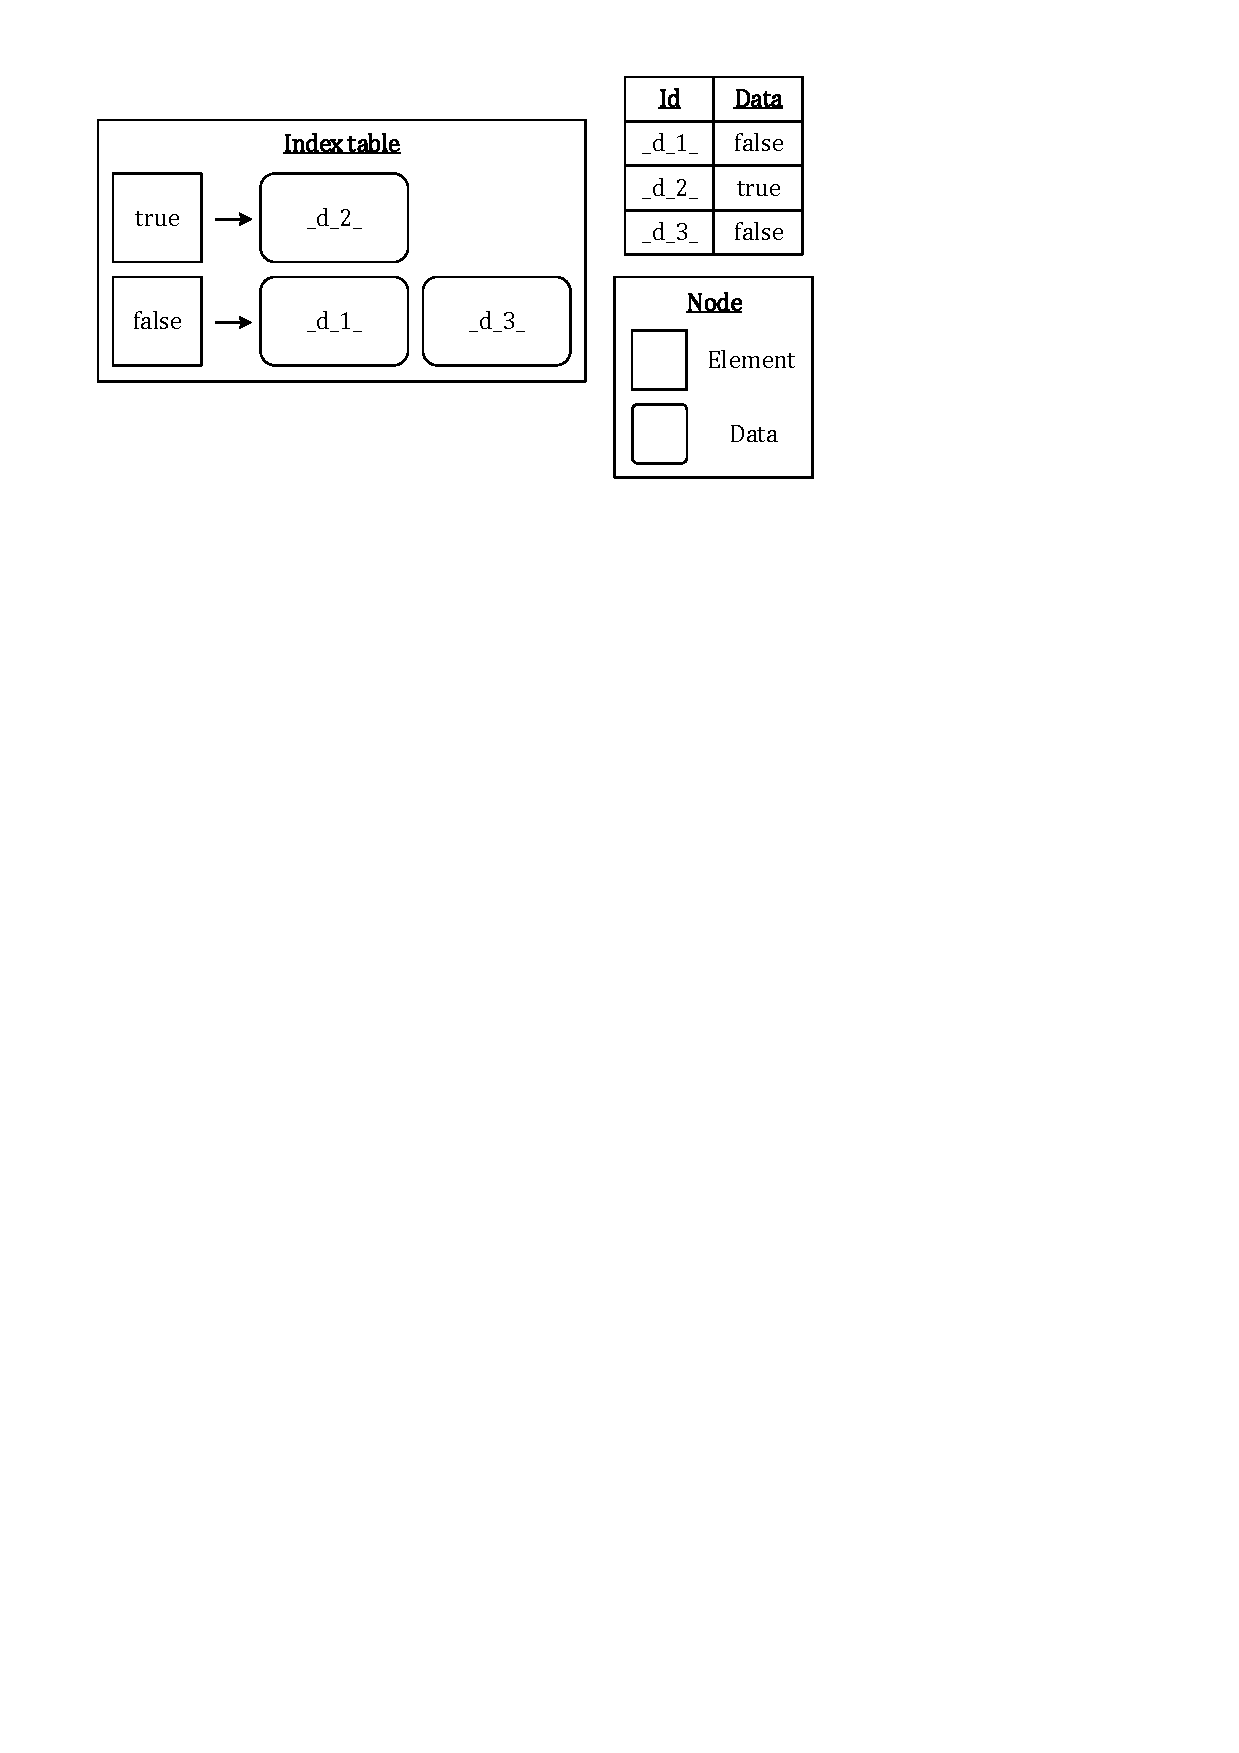
\includegraphics[scale=0.8]{./algorithm/boolean/pic/example_1_v1.pdf}
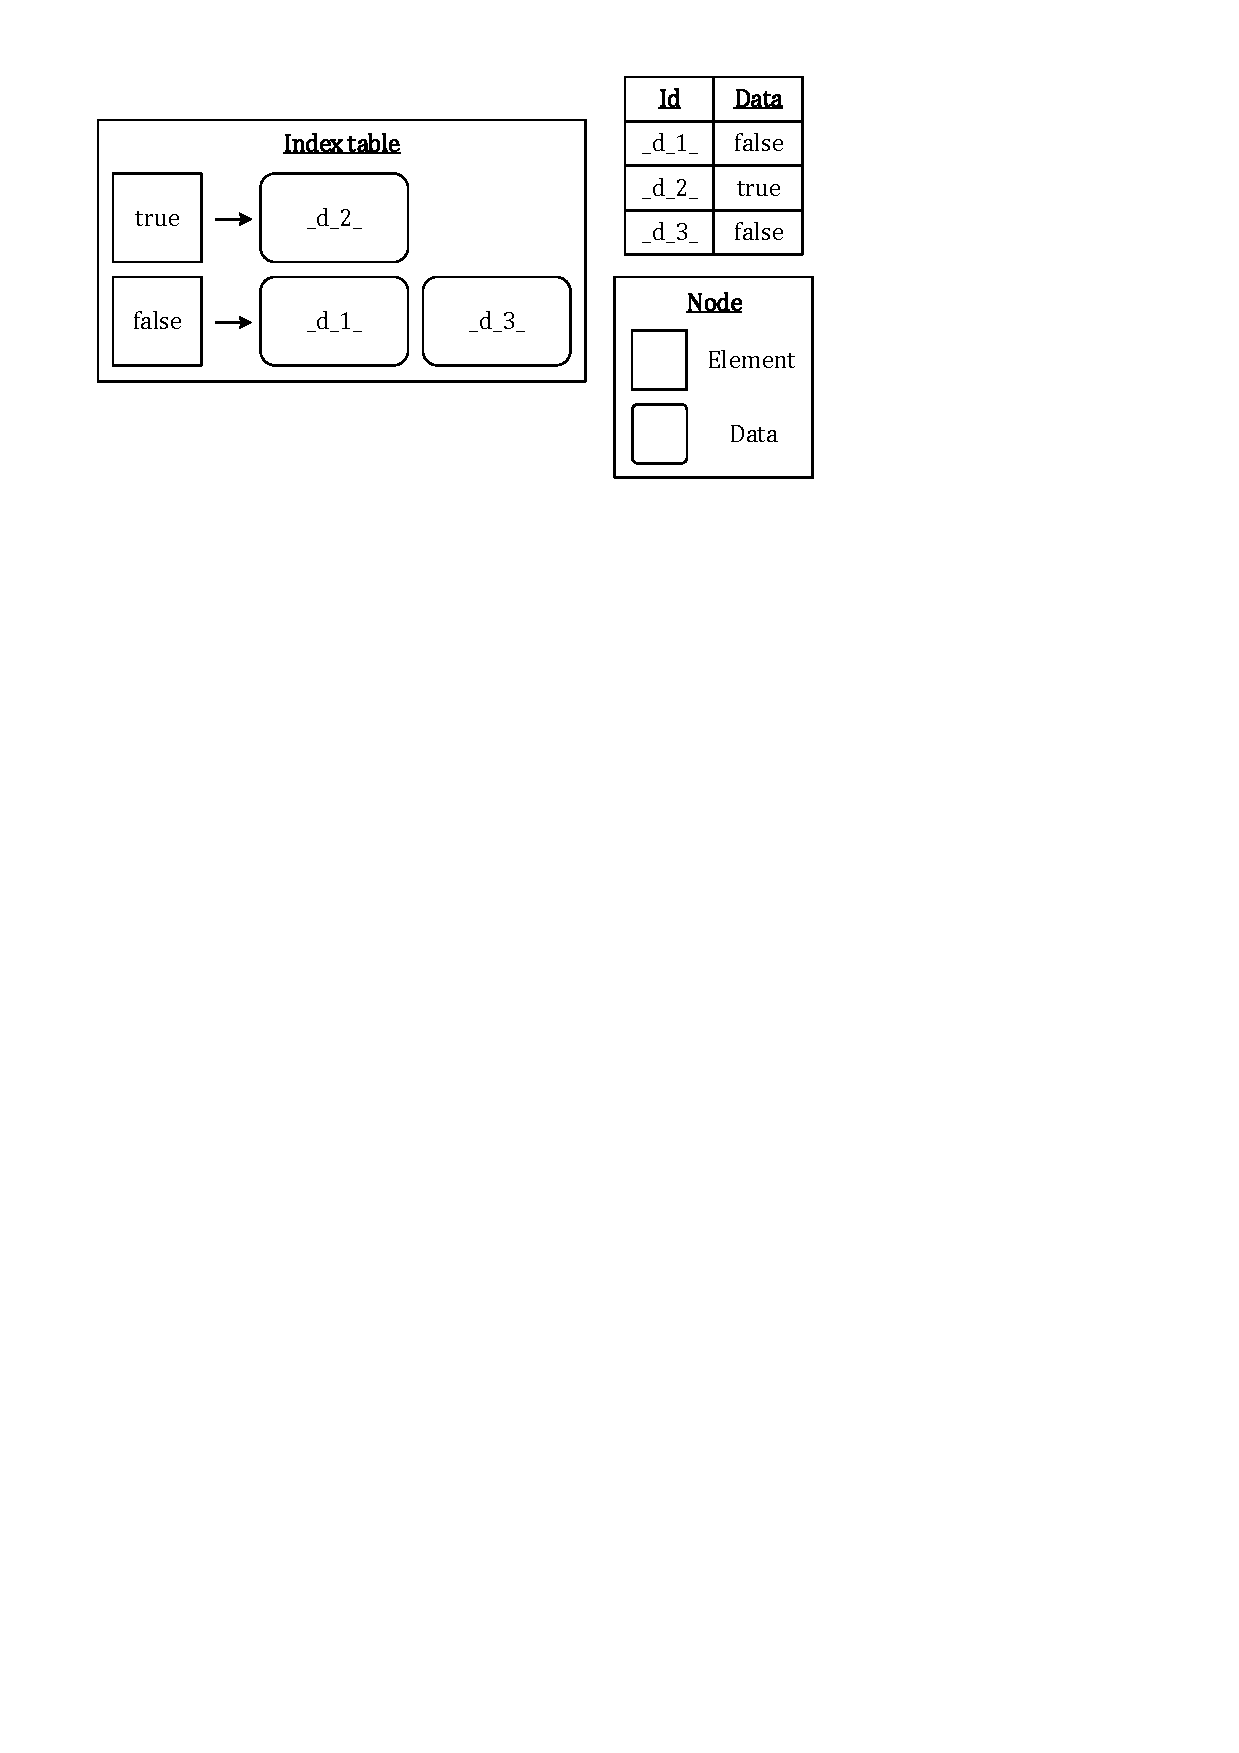
\includegraphics[width=0.8\textwidth]{./algorithm/boolean/pic/example_1_v1.pdf}
\caption{The indexing tables of in \textit{BOOLEAN} type.}
\label{fig:algorithm:boolean:example_1}
\end{figure}


% Insertion section
\subsubsection{Insertion}

When inserting a new data, it just need to add the data node into the bucket where the data belong with, so the time complexity should be $O(1)$.


% Deletion section
\subsubsection{Deletion}

Delete a data node is just get the bucket and remove the data node, so this is also a quick operation where time complexity be $O(1)$.


% Modification section
\subsubsection{Modification}

Modify the data is actually delete the node in a bucket and re-insert it again into another bucket. Time complexity should be $O(1)$.



% Selection section
\subsubsection{Selection}

Select operation is the simplest operation than the other, because the selection for \textit{BOOLEAN} type is only can select $"true"$ or $"false"$, so select the bucket then this will return the whole bucket, so this is also a quick operation. Also if user want to retrieve all, just retrieve both $"true"$ and $"false"$ bucket will get all data. That time complexity of both searching are $O(1)$.


% Summary section
\subsubsection{Summary}

Table \ref{table:algorithm:boolean:summary:time_complexity} is summarized the time complexity of each opration in \textit{BOOLEAN} type.

\begin{table}[h]
\centering
\caption{Time complexity for \textit{BOOLEAN} type.}
\label{table:algorithm:boolean:summary:time_complexity}
\begin{tabular}{|c|c|}

\hline
\multicolumn{1}{|c|}{Operation} &
\multicolumn{1}{c|}{Time complexity} \\

\hline
\multicolumn{1}{|c|}{Insert} &
\multicolumn{1}{c|}{$O(1)$} \\

\hline
\multicolumn{1}{|c|}{Modify} &
\multicolumn{1}{c|}{$O(1)$} \\

\hline
\multicolumn{1}{|c|}{Delete} &
\multicolumn{1}{c|}{$O(1)$} \\

\hline
\multicolumn{1}{|c|}{Selection} &
\multicolumn{1}{c|}{$O(1)$} \\

\hline
\end{tabular}
\end{table}


\clearpage
